\chapter{Artificial intelligence \& Machine Learning}

Machine learning is a branch of \Gls{ai}. 
The field of \Gls{machinevision} is a branch of machine vision in which important steps forward has been made in the past decade, mainly thanks to the emergence of \Gls{deepl}.

The aim of this chapter is not to provide a complete overview of the machine learning field.
Rather, the objective is to highlight concepts that are important for interpretation of the specific analysis in this Master thesis.

\section{Birds-eye view on the field of Artificial Intelligence}

The field of \Gls{ai} (AI) is the engineering discipline of the automation of \textit{cognitive} tasks.
Tasks such as search, control and classification are generally considered to require a level of intelligence. 
Automation of this type of tasks to allow a machine to perform them is thus \Gls{ai}\footnote{To be precise, it is not the human intelligence that is replicated. It is the \textit{effect} of this intelligence.}.
A classic PID controller and even a bang-bang (thermostat) controller can be viewed as simple, but very effective, forms of AI.


In the past decades, this engineering discipline has incredible advance, driven both by leaps forward in the available hardware and the development of new algorithms and models. \\
First, the availability and reliability of hardware components such as sensors, cameras, digital storage and calculation power has increased exponentially 
\footnote{ \textit{Moore's law} states that the number of transistors on an integrated curcuit doubles every two years. This rate of progress has held more of less for a wide range of digital components in the past decades.}.
The size and price of these components has decreased equally dramatically. \\
Second, important progress has been made in the development of algorithms to make use of this available data and computation power to solve problems and perform tasks.
I do not want to provide a complete overview of all existing machine learning models. 
In this work, I make use of \Gls{deepl} models.
A \Gls{deepl} model is a type of \acrfull{ann} with multiple hidden layers. 
Deep learning models are behind almost all modern applications of \acrfull{nlp} and \Gls{machinevision}.

Deep learning models can be fitted through the \acrfull{bp} algorithm. 
\todo[inline]{Short and to-the point introduction of neural networks}

\section{Losses and metrics}

Constructing a network requires evaluating it, comparing the evaluation output to a known desired output and trying to take steps to bring the model output closer to the desired output. 
A network is fitted to the \textit{train set} by the optimization algorithm, based on the \textbf{loss}.
The \acrshort{ml} engineer wants to judge the performance of the model based on one or several \textbf{metrics}, calculated on the \textit{train set}, the \textit{cross-validation set} and eventually on the \textit{test set}.

\section{Machine vision}

\Gls{machinevision} is the branch of \Gls{ai} focussed on image processing.
The machine vision task performed in this work is called instance \Gls{segmentation}.
In this chapter, I explain what this means. 
I compare segmentation to other machine vision tasks.

This work investigates the use of \Gls{weaklysupervisedl} data for training an Instance segmentation model. 
I explain the concept and benefits of \Gls{weaklysupervisedl} machine learning.

\subsection{Machine vision tasks \label{sec:machinevisiontasks}}

\Gls{machinevision} is a broad discipline. 
Humans extract information from images almost subconsciously, and we are often not aware of the different tasks we perform on images.
The objective of this section is to briefly define different machine vision tasks discussed further in this book. 
Several machine vision tasks consist of \textit{recognizing} objects, animals or humans in an image.
A model is built for a finite list of \textit{categories} that can be present in an image.
Depending on the question asked ad inference time, one can distinguish the following tasks.

\begin{description}
    \item[Image classification] is the task of determining what object category\footnote{or categories} is present in the image. Is there a cat in this image?
    \item[Object counting] is the task of counting how many instances of each category are in the image. How many cats are there in this picture? 
    \item[Object detection] consists not only of identification of the object. Also, the spatial position is requested, often in the form of a bounding box. Where is the cat in this picture if a cat is present?
    \item[Semantic segmentation] requires a class estimation for each image pixel. Pixels that do not belong to a specific class are called the \textit{background}.
    \item[Instance segmentation] requires not only that the semantic class determined for each pixel, but also that two individuals of the same class\footnote{say, two cats.} are distinguished.   
\end{description}

Figure \ref{fig:machinevisiontasks} illustrates the difference between these machine vision tasks. 

\begin{SCfigure}[][h!]
    \centering
    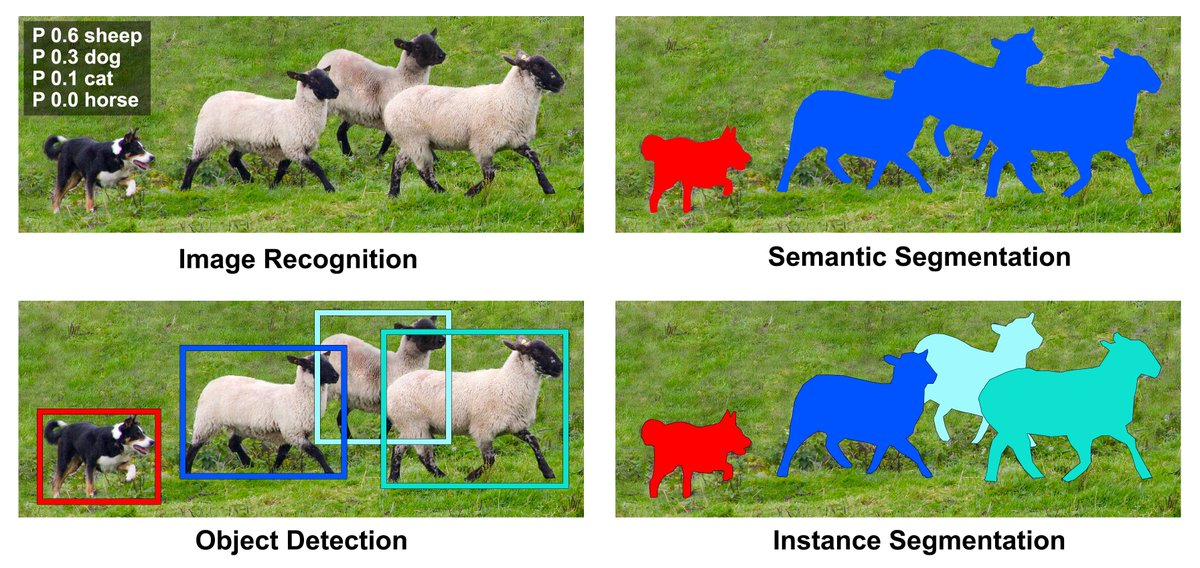
\includegraphics[width=10cm]{/home/thesis/images/Classification_vs_Segmentation.jpg}
    \caption{Illustration to compare different Machine vision tasks \cite{SemTorch76:online}. 
    Object detection means that the location of several objects is estimated by the model. This is indicated by the \textit{bounding boxes}.
    Segmentation of an image is classifying each pixel in the correct class or assigning it to the \textit{background} class.
    Semantic segmentation makes no difference between different instances of the same semantic class, instance segmentation does.
    \label{fig:machinevisiontasks}}
\end{SCfigure}

Other interesting applications of \gls{machinevision} include\footnote{This list is not exhaustive.}:
\begin{description}
    \item[Face recognition] is the identification of human faces. 
    \item[Image reconstruction] or \textit{inpainting} consists of recreating parts of a damaged image.
    \item[Image captioning] consists of the creation of full sentences describing the content of an image.    
\end{description}

\subsection{The convolution layer}

The building block of every modern machine vision network, including the ones in my thesis, is the convolution layer.

\todo[inline]{weight sharing, feature extraction}

\subsection{Data for training a machine vision model}

To perform the tasks discussed in chapter \ref{sec:machinevisiontasks}, one needs to build a suitable model.
For \Gls{machinevision} tasks\footnote{and many other tasks.}, the current standard approach is \Gls{deepl}.


The cost to generate, store and communicate images and computation power has dropped in the past decades.
This evolution allows to train a model  on previously unimaginable quantities of data\footnote{The \textit{ImageNet} database (\url{http://image-net.org/challenges/LSVRC/index}) consists of more than $14.10^6$ images.}.
This technique allows a model with a high number of degrees of freedom to be trainded\footnote{learn by example, so you will} without the need for expert-crafted features. 


Collection of this dataset - most importantly, the labels - proves to be a challenge. 
This chapter tries to explain what \textit{weak labels} and \textit{strong labels} are and what the difference is between both.

\subsubsection{Training a model}

To build a model to perform the tasks discussed in \ref{sec:machinevisiontasks}, this model needs to be trained.
This requires a set of \textit{labelled} images. 

In the classic approach, the supervision type closely resembles the intended model output.
To train a model that can classify an image\footnote{Given an image, the model outputs if this picture is a representation of class \textit{cat}, \textit{dog} or another animal or object. }, 
one has to \textit{train} the model on a set of labelled images where a human indicated the class.
To train a model to perform image segmentation\footnote{segmentation means that the model classifies each pixel.}, an expert needs to provide a set of images in which
each picture, the objects are delineated, indicating their class.  



\subsubsection{Weak supervision types}


To build a machine vision model, a collection of images is needed where an expert in the intended task has provided correct information from which the model can \textit{learn}.
Depending on the model objective, other types of labelling are required.


Figure \ref{fig:ImageLabelTypes} illustrates several types of image supervision : 
Point supervision, squiggle, bounding box and full mask.
The generation of these labels is costly and time-consuming.
Especially \gls{deepl} models are known to be very data-hungry. 

\begin{SCfigure}[][htb]
    \centering
    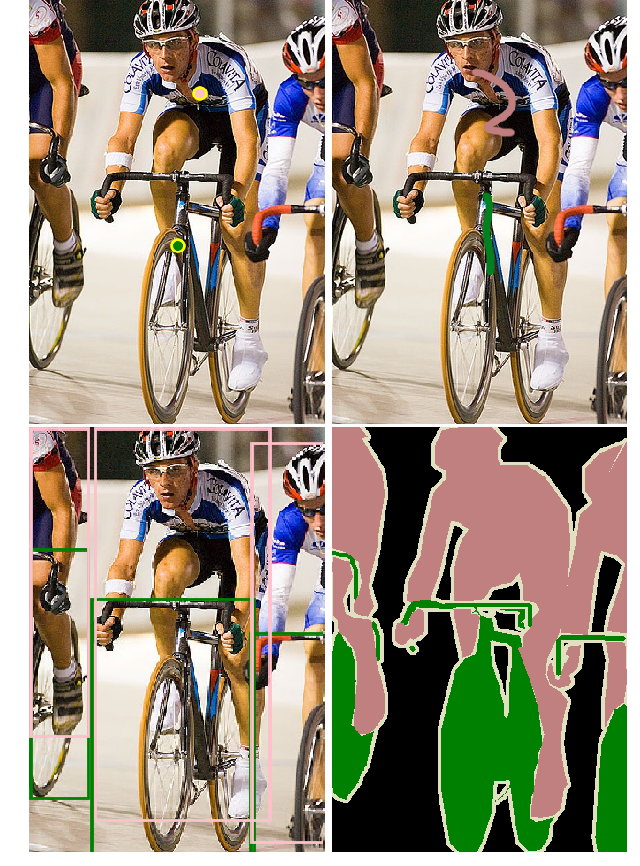
\includegraphics[width=10cm]{/home/thesis/images/McEver.png}
    \caption{Four different annotation types \cite{McEver2020}: 
    On the top left the picture is point level annotated. The points are inflated for visibility.
    On the top right, squiggle annotation is used.
    The bottom left shows bounding box supervion.
    While the bottom right image is fully annotated.
    An image level label would indicate that there are multiple instances of \textit{person} and \textit{bike} in the image.
    \label{fig:ImageLabelTypes}}
\end{SCfigure}

Given the high labelling cost, several researchers have investigated ways to train computer vision models with cheaper labels.
This branch of research is known as \Gls{weaklysupervisedl}.
The objective is to construct a robust model based on \textit{cheap} (incomplete, noisy or imprecise) labels. 
This is sometimes described as \textit{indirect supervision}.
Numerous creative approaches have been conceived. 
It is impossible to give an exhaustive list of approaches. 
In what follows, I will mainly focus on the approaches I chose to investigate myself, but I will also try to give some hints of the remarkable creativity found in the field.
Since the provided annotations in \Gls{weaklysupervisedl} are not full labels, these are sometimes described as \textit{hints} instead\footnote{
    This is based on the insightfull talk at \url{ 
        https://youtu.be/4EjYxVVCAaE
    }. For example, the destinction between labels and hints.
}.
The basic concept of \Gls{weaklysupervisedl} is that there are two sources of information to draw from: The hints and the prior knowledge about the problem (Priors).
These \textit{Priors} can be any form of prior knowledge about the object to be segmented\footnote{or any other machine vision task.}.
Priors can be the object size, shape or location, the number of instances, the similarity across images or the similarity with external images.

Whether an annotation is considered a \textit{weak label} or a \textit{strong label} depends more on the modellers intention than on the annotation itself. 
When one aims to construct a model to infer output labels with a higher informative value than the original annotations, these \textit{labels} become \textit{hints}.
Making a model predict bounding boxes from a dataset annotated with bounding boxes means considering these as \textit{strong labels}. 
If one uses the same dataset to construct a model that predicts pixel-wise masks, you use the labels as \textit{weak labels} or \textit{hints}.

For a segmentation task, weak labels can be:
\begin{description}
    \item[Image level labels]: When only  
\end{description}

\todo[inline]{Motivation of weakly supervised learning --> Difference in annotation time and cost from Bearman and Laradji Covid}